\section{Methods}\label{sec:methods}
In this chapter we are clarifying the Loss and Metric Functions, the Architecture BERT used for our Experiments, Ideas principles like Adapter Tuning and
Sentence Embedding and how fusing different Dataset together works, which are used in training loop.


\subsection{BERT}
\begin{figure}[b]
    \vspace{-1cm}
    \centering
    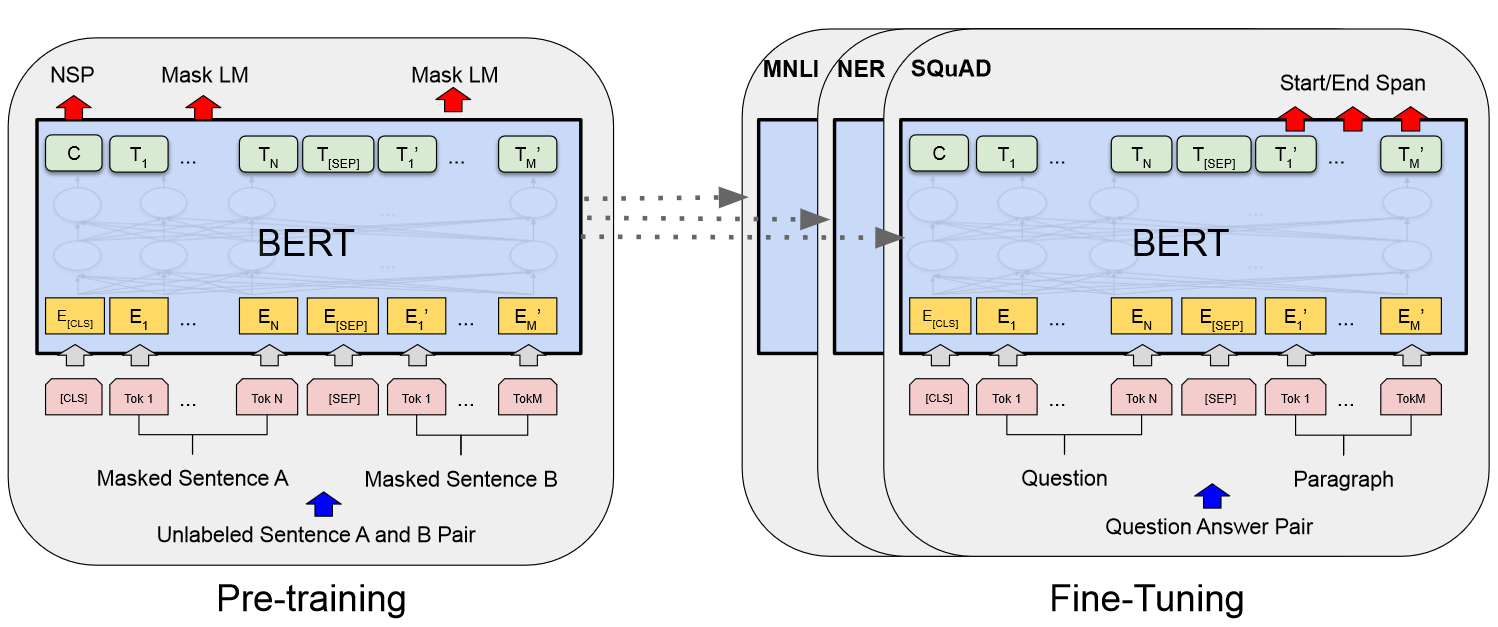
\includegraphics[scale=0.22]{./content/BERT_Architecture.png}
    \caption{Bidirectional Encoder Representations from Transformers (BERT) 
             schematic View \cite{devlin_bert_2019}.}
    \label{tab:bert}
\end{figure}

The Experiments are using BERT, Bidirectional Encoder Representations from Transformers (see Figure~\ref{tab:bert}) ~\cite{devlin_bert_2019} 
developed by Google is based on Transformer architecture introduced by Vaswani et al. \cite{vaswani_attention_2023}.
Unlike previous attempts, that process text in a unidirectional way (either left to right or right to 
left), BERT is designed to understand context bidirectionally as every Token is connected Pathways with every other. A masked language model (MLM) 
pre-training target is used, where tokens are randomly masked from the input to predict the original 
vocabulary IDs.
The model can be fine-tuned for specific downstream tasks, such as classification or translation. 
BERT is available in different sizes like BERT-Base and BERT-Large. There are various implementations 
such as RoBERTa~\cite{liu_roberta_2019}, ALBERT~\cite{lan_albert_2020}, BART~\cite{lewis_bart_2020}, 
DeBERTa~\cite{he_deberta_2021}, which improves BERT architecture differently.

We are using pre-trained BERT-Base Model from Huggingface~\cite{noauthor_hugging_2024-1} due to Limitations
of the Environment (see Chapter~\ref{ch:ev}) and supervised fine-tune it to SemEval.














\subsection{Sentence Embedding Architectures}\label{ch:seb}
\begin{figure}[!b]
    \vspace{-1cm}
    \centering
    %\resizebox{\textwidth}{!}{\begin{tikzpicture}
	\begin{pgfonlayer}{nodelayer}
		\node [style=rec] (0) at (0, 0) {Bert};
		\node [style=Textfeld] (1) at (0, 2) {Sentence};
		\node [style=rec] (2) at (0, -0.5) {For};
		\node [style=rec] (4) at (0, -1) {Sentence};
		\node [style=rec] (5) at (0, -1.5) {Classification};
		\node [style=Textfeld] (9) at (2.75, 2) {smt};
		\node [style=Textfeld] (10) at (4.25, 2) {sec};
		\node [style=Textfeld] (11) at (5.75, 2) {$p_1, p_2, ...$};
		\node [style=Textfeld] (12) at (7.25, 2) {$s_1, s_2, ...$};
		\node [style=Scale] (13) at (5, -2) {Cat(u, v, x, y)};
		\node [style=Softmax] (14) at (5, -2.75) {Classifier};
		\node [style=Linear] (15) at (2.75, 0) {BERT};
		\node [style=Linear] (16) at (4.25, 0) {BERT};
		\node [style=Linear] (17) at (5.75, 0) {BERT};
		\node [style=Linear] (18) at (7.25, 0) {BERT};
		\node [style=Textfeld] (19) at (0, -4) {0 or 1};
		\node [style=Textfeld] (20) at (5, -4) {0 or 1};
		\node [style=Textfeld] (21) at (11.25, 2) {smt};
		\node [style=Textfeld] (22) at (12.75, 2) {$s_1, s_2, ...$};
		\node [style=Textfeld] (23) at (12.75, 2.5) {$p_1, p_2, ...$};
		\node [style=Scale] (25) at (9.5, -2) {Cat(u, v)};
		\node [style=Softmax] (26) at (9.5, -2.75) {Classifier};
		\node [style=Linear] (27) at (11.25, 0) {BERT};
		\node [style=Linear] (28) at (12.75, 0) {BERT};
		\node [style=Textfeld] (31) at (9.5, -4) {0 or 1};
		\node [style=Textfeld] (32) at (12.75, 3) {sec};
		\node [style=Scale] (36) at (12, -2) {Cat(u, v, |u-v|)};
		\node [style=Softmax] (37) at (12, -2.75) {Classifier};
		\node [style=Textfeld] (40) at (12, -4) {0 or 1};
		\node [style=Scale] (45) at (14.5, -2) {CosSim(u, v)};
		\node [style=Softmax] (46) at (14.5, -2.75) {Map(-1, 1 -> 0, 1)};
		\node [style=Textfeld] (49) at (14.5, -4) {0 or 1};
		\node [style=none] (51) at (1.75, 3) {};
		\node [style=none] (52) at (1.75, -5.25) {};
		\node [style=none] (53) at (8.25, 3) {};
		\node [style=none] (54) at (8.25, -5.25) {};
		\node [style=Textfeld] (55) at (0, -5) {\textbf{v1/Baseline}};
		\node [style=Textfeld] (56) at (5, -5) {\textbf{v2}};
		\node [style=Textfeld] (57) at (9.5, -5) {\textbf{v3}};
		\node [style=Textfeld] (58) at (12, -5) {\textbf{v4}};
		\node [style=Textfeld] (59) at (14.5, -5) {\textbf{v5/v6}};
		\node [style=none] (60) at (-1.25, -4.5) {};
		\node [style=none] (61) at (16, -4.5) {};
	\end{pgfonlayer}
	\begin{pgfonlayer}{edgelayer}
		\draw [style=arrow] (1) to (0);
		\draw [style=arrow] (13) to (14);
		\draw [style=arrow] (9) to (15);
		\draw [style=arrow] (15) to (13);
		\draw [style=arrow] (16) to (13);
		\draw [style=arrow] (10) to (16);
		\draw [style=arrow] (11) to (17);
		\draw [style=arrow] (17) to (13);
		\draw [style=arrow] (12) to (18);
		\draw [style=arrow] (18) to (13);
		\draw [style=arrow] (5) to (19);
		\draw [style=arrow] (14) to (20);
		\draw [style=arrow] (25) to (26);
		\draw [style=arrow] (21) to (27);
		\draw [style=arrow] (27) to (25);
		\draw [style=arrow] (28) to (25);
		\draw [style=arrow] (22) to (28);
		\draw [style=arrow] (26) to (31);
		\draw [style=arrow] (36) to (37);
		\draw [style=arrow] (37) to (40);
		\draw [style=arrow] (45) to (46);
		\draw [style=arrow] (46) to (49);
		\draw (51.center) to (52.center);
		\draw [style=arrow] (27) to (36);
		\draw [style=arrow] (27) to (45);
		\draw [style=arrow] (28) to (36);
		\draw [style=arrow] (28) to (45);
		\draw (53.center) to (54.center);
		\draw (60.center) to (61.center);
	\end{pgfonlayer}
\end{tikzpicture}
}
    \resizebox{\textwidth}{!}{\begin{tikzpicture}
	\begin{pgfonlayer}{nodelayer}
		\node [style=rec] (0) at (0, 0) {Bert};
		\node [style=Textfeld] (1) at (0, 2) {Sentence};
		\node [style=rec] (2) at (0, -0.5) {For};
		\node [style=rec] (4) at (0, -1) {Sentence};
		\node [style=rec] (5) at (0, -1.5) {Classification};
		\node [style=Textfeld] (9) at (2.75, 2) {smt};
		\node [style=Textfeld] (10) at (4.25, 2) {sec};
		\node [style=Textfeld] (11) at (5.75, 2) {$p_1, p_2, ...$};
		\node [style=Textfeld] (12) at (7.25, 2) {$s_1, s_2, ...$};
		\node [style=Scale] (13) at (5, -2) {Cat(u, v, x, y)};
		\node [style=Softmax] (14) at (5, -2.75) {Classifier};
		\node [style=Linear] (15) at (2.75, 0) {BERT};
		\node [style=Linear] (16) at (4.25, 0) {BERT};
		\node [style=Linear] (17) at (5.75, 0) {BERT};
		\node [style=Linear] (18) at (7.25, 0) {BERT};
		\node [style=Textfeld] (19) at (0, -4) {0 or 1};
		\node [style=Textfeld] (20) at (5, -4) {0 or 1};
		\node [style=Textfeld] (21) at (11.25, 2) {smt};
		\node [style=Textfeld] (22) at (12.75, 2) {$s_1, s_2, ...$};
		\node [style=Textfeld] (23) at (12.75, 2.5) {$p_1, p_2, ...$};
		\node [style=Scale] (25) at (9.5, -2) {Cat(u, v)};
		\node [style=Softmax] (26) at (9.5, -2.75) {Classifier};
		\node [style=Linear] (27) at (11.25, 0) {BERT};
		\node [style=Linear] (28) at (12.75, 0) {BERT};
		\node [style=Textfeld] (31) at (9.5, -4) {0 or 1};
		\node [style=Textfeld] (32) at (12.75, 3) {sec};
		\node [style=Scale] (36) at (12, -2) {Cat(u, v, |u-v|)};
		\node [style=Softmax] (37) at (12, -2.75) {Classifier};
		\node [style=Textfeld] (40) at (12, -4) {0 or 1};
		\node [style=Scale] (45) at (14.5, -2) {CosSim(u, v)};
		\node [style=Softmax] (46) at (14.5, -2.75) {Map(-1, 1 -> 0, 1)};
		\node [style=Textfeld] (49) at (14.5, -4) {0 or 1};
		\node [style=none] (51) at (1.75, 3) {};
		\node [style=none] (52) at (1.75, -5.25) {};
		\node [style=none] (53) at (8.25, 3) {};
		\node [style=none] (54) at (8.25, -5.25) {};
		\node [style=Textfeld] (55) at (0, -5) {\textbf{v1/Baseline}};
		\node [style=Textfeld] (56) at (5, -5) {\textbf{v2}};
		\node [style=Textfeld] (57) at (9.5, -5) {\textbf{v3}};
		\node [style=Textfeld] (58) at (12, -5) {\textbf{v4}};
		\node [style=Textfeld] (59) at (14.5, -5) {\textbf{v5/v6}};
		\node [style=none] (60) at (-1.25, -4.5) {};
		\node [style=none] (61) at (16, -4.5) {};
	\end{pgfonlayer}
	\begin{pgfonlayer}{edgelayer}
		\draw [style=arrow] (1) to (0);
		\draw [style=arrow] (13) to (14);
		\draw [style=arrow] (9) to (15);
		\draw [style=arrow] (15) to (13);
		\draw [style=arrow] (16) to (13);
		\draw [style=arrow] (10) to (16);
		\draw [style=arrow] (11) to (17);
		\draw [style=arrow] (17) to (13);
		\draw [style=arrow] (12) to (18);
		\draw [style=arrow] (18) to (13);
		\draw [style=arrow] (5) to (19);
		\draw [style=arrow] (14) to (20);
		\draw [style=arrow] (25) to (26);
		\draw [style=arrow] (21) to (27);
		\draw [style=arrow] (27) to (25);
		\draw [style=arrow] (28) to (25);
		\draw [style=arrow] (22) to (28);
		\draw [style=arrow] (26) to (31);
		\draw [style=arrow] (36) to (37);
		\draw [style=arrow] (37) to (40);
		\draw [style=arrow] (45) to (46);
		\draw [style=arrow] (46) to (49);
		\draw (51.center) to (52.center);
		\draw [style=arrow] (27) to (36);
		\draw [style=arrow] (27) to (45);
		\draw [style=arrow] (28) to (36);
		\draw [style=arrow] (28) to (45);
		\draw (53.center) to (54.center);
		\draw (60.center) to (61.center);
	\end{pgfonlayer}
\end{tikzpicture}
}
    \caption{Sentence Embedding idea is based on BERT Model. Strategy v1 is the
             Baseline, handling everything in once and every token can contribute to each other, while
             Strategy v2 split the sentence in four parts, and fed separately to the same
             model. Strategy v3, v4, v5 and v6
             uses the same idea but Concatenating, using only premise and hypothesis and generating the output differently.}\label{fig:ver}
\end{figure}

Sentence-BERT (SBERT) \cite{reimers_sentence-bert_2019}, a modification of the BERT \cite{devlin_bert_2019} network, is a strategy designed for 
semantic similarity tasks, to generate meaningful embeddings. While BERT \cite{devlin_bert_2019} and RoBERTa \cite{liu_roberta_2019} excel in sentence-pair 
regression tasks, they suffer from computational overhead when dealing with large 
collections of sentences. SBERT addresses this issue by using 
siamese and triplet network structures to generate semantically meaningful 
sentence embeddings. Also, a key point is, especially with BERT, the two sentences are 
passing the Model individual, meaning that the Tokens of each sentence does not interfere
with each other. This allows for efficient similarity comparisons, 
clustering, and semantic search.
The authors demonstrate that SBERT significantly reduces the time required for 
finding the most similar pair in a collection of 10,000 sentences from 65 
hours with BERT to about 5 seconds.

We use this Principle and applied it to the SemEval Task (see Figure~\ref{fig:ver}). 
Therefore, we come up with five different ideas, where they use the Siamese-Architecture as Core, 
which is sharing the Models Parameters. Version-2 (v2) has four
parts of the defined Sentence (see Equation~\ref{eq:ds-sentence}) split at the $[SEP]$ Tokens.
Version-3 (v3), Version-4 (v4), Version-5 (v5) and Version-6 (v6) has the split on the first $[SEP]$ Token, to separate Statement from the Hypothesis.
Version-3 and Version-4 uses a simple Feed-Forward-Classifier after the Concatenation combined with CrossEntropyLoss.
Version-5 and Version-6 uses Cosine Similarity, with a Mapping ensuring Entailment being $1$ and
Contradiction being $-1$. Version-5 uses CosineEmbeddingLoss and Version-6 uses MSELoss to 
minimize, if entailed, and maximize, if contradiction, the spatial distances.


















\subsection{Adapter Tuning}\label{ch:adapter}

Adapter Tuning (see Figure~\ref{tab:adapt}) is a supervised method, where input, gold label are given and the models parameters are frozen, 
but adding new fully trainable bottleneck feed-forward networks 
on each intermediate layer. The objective is to reduce the size of trainable parameters, 
to gain higher throughput and keeping the pre-trained embeddings\cite{zheng_learn_2023} \cite{naveed_comprehensive_2023}. 
The ultimate goal of adaptation training is to enhance the model's scores on the downstream task, 
while still benefiting from the broad language understanding gained during the initial 
pre-training \cite{manjavacas_adapting_2022}. The effectiveness of adaptation-tuning depends on 
the similarity between the pre-training task and the target task due to fixed embeddings.

\begin{figure}[!b]
    \centering
    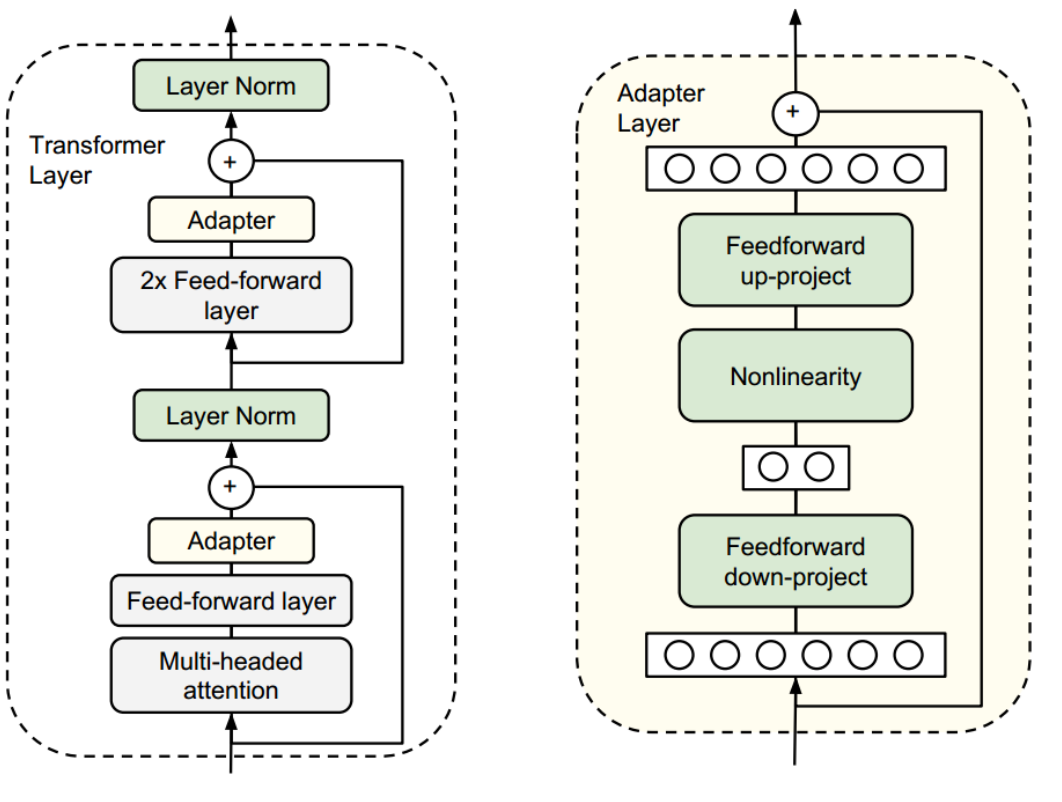
\includegraphics[scale=0.28]{./content/Adapter_Architecture.png}
    \caption{Basic Structure of Adapter built on top of a Models Architecture (left side), where only the Adapter Layers Parameters (right side) are trainable \cite{zheng_learn_2023}.
             In our Case we are using $768$ to $512$ Down-Projector, followed by GELU-Activation and
             $512$ to $768$ UP-Projector.}
    \label{tab:adapt}
\end{figure}


For our Experiments we are comparing supervised fine-tuned BERT, with the SemEval dataset against
a Adapter-BERT version, where the pre-trained BERT's Parameters are frozen. Secondly we are
taking the BERT Model from SimCSE~\cite{gao_simcse_2022-1}, which applied a Supervised
Contrastive Learning idea on SNLI Data, to minimize and maximize the spatial distances,
which effects the Output Representations of BERT and using the same principle with the Adapter on this Model.







\subsection{Loss Functions and Evaluation Metric}
We are using 3 commonly used Loss functions for our Training of the different
Architectures with $x$ being the Prediction and $y$ being the searched Class. For direct Classification, 
CrossEntropyLoss~\ref{eq:ce} is the commonly and most frequently used function. Secondly, as we see later,
combined with Cosine Simmilarity, we are using MSELoss~\ref{eq:mse} or CosineEmbeddingLoss~\ref{eq:ceb}
to maximize or minimize the distance between two representations. As Metric the SemEval Task uses F1 Score, which
is the harmonic mean between precision and recall defined in Equation~\ref{eq:f} \cite{noauthor_nli4ct_nodate}.



\begin{equation}\label{eq:ce}
   Loss_{CE} = -\sum_{i=1}^My_{o,i}\log(x_{o,i})
\end{equation}
\begin{equation}\label{eq:mse}
   Loss_{MSE} = \sum_{i=1}^{M}(x_i-y_i)^2
\end{equation}

\begin{equation}\label{eq:ceb}
    Loss_{CEB} = \begin{cases}
        1 - \cos(x_1, x_2),      &\text{if $y = +1$}\\
        \max(0, \cos(x_1, x_2)), &\text{if $y = -1$}
    \end{cases}
\end{equation}

\begin{equation}\label{eq:f}
    F_1 = 2 \frac{precision \cdot recall}{precision + recall} = \frac{2 TP}{2TP + FP + FN}
 \end{equation}


 



\subsection{Fusing different Datasets/Loaders}
\begin{figure}[b]
    \centering
    \resizebox{\textwidth}{!}{\begin{tikzpicture}
	\begin{pgfonlayer}{nodelayer}
		\node [style=base] (0) at (0, 0) {};
		\node [style=1x1 v1] (1) at (-7.5, 0) {};
		\node [style=1x1 v1] (4) at (-6.5, 0) {};
		\node [style=1x1 v1] (6) at (-5.5, 0) {};
		\node [style=1x1 v1] (7) at (-4.5, 0) {};
		\node [style=1x1 v3] (9) at (-3.5, 0) {};
		\node [style=1x1 v3] (10) at (-2.5, 0) {};
		\node [style=1x1 v3] (11) at (-1.5, 0) {};
		\node [style=1x1 v3] (12) at (-0.5, 0) {};
		\node [style=1x1 v4] (35) at (0.5, 0) {};
		\node [style=1x1 v4] (36) at (1.5, 0) {};
		\node [style=1x1 v4] (37) at (2.5, 0) {};
		\node [style=1x1 v4] (38) at (3.5, 0) {};
		\node [style=1x1 v2] (39) at (4.5, 0) {};
		\node [style=1x1 v2] (40) at (5.5, 0) {};
		\node [style=1x1 v2] (41) at (6.5, 0) {};
		\node [style=1x1 v2] (42) at (7.5, 0) {};
		\node [style=base] (43) at (19, 0) {};
		\node [style=1x1 v1] (44) at (11.5, 0) {};
		\node [style=1x1 v1] (45) at (12.5, 0) {};
		\node [style=1x1 v1] (46) at (13.5, 0) {};
		\node [style=1x1 v1] (47) at (14.5, 0) {};
		\node [style=1x1 v3] (48) at (15.5, 0) {};
		\node [style=1x1 v3] (49) at (16.5, 0) {};
		\node [style=1x1 v4] (52) at (17.5, 0) {};
		\node [style=1x1 v2] (56) at (19.5, 0) {};
		\node [style=1x1 v2] (57) at (24.5, 0) {};
		\node [style=1x1 v2] (58) at (25.5, 0) {};
		\node [style=1x1 v2] (59) at (26.5, 0) {};
		\node [style=base] (60) at (0, -3) {};
		\node [style=1x1 v1] (61) at (-7.5, -3) {};
		\node [style=1x1 v1] (62) at (-6.5, -3) {};
		\node [style=1x1 v1] (63) at (-5.5, -3) {};
		\node [style=1x1 v1] (64) at (-4.5, -3) {};
		\node [style=1x1 v3] (65) at (-3.5, -3) {};
		\node [style=1x1 v3] (66) at (-2.5, -3) {};
		\node [style=1x1 v3] (67) at (-1.5, -3) {};
		\node [style=1x1 v3] (68) at (-0.5, -3) {};
		\node [style=1x1 v4] (69) at (0.5, -3) {};
		\node [style=1x1 v4] (70) at (1.5, -3) {};
		\node [style=1x1 v4] (71) at (2.5, -3) {};
		\node [style=1x1 v4] (72) at (3.5, -3) {};
		\node [style=1x1 v2] (73) at (4.5, -3) {};
		\node [style=1x1 v2] (74) at (5.5, -3) {};
		\node [style=1x1 v2] (75) at (6.5, -3) {};
		\node [style=1x1 v2] (76) at (7.5, -3) {};
		\node [style=base] (77) at (0, -1.5) {};
		\node [style=1x1 v1] (78) at (-7.5, -1.5) {};
		\node [style=1x1 v1] (79) at (-6.5, -1.5) {};
		\node [style=1x1 v1] (80) at (-5.5, -1.5) {};
		\node [style=1x1 v1] (81) at (-4.5, -1.5) {};
		\node [style=1x1 v3] (82) at (-3.5, -1.5) {};
		\node [style=1x1 v3] (83) at (-2.5, -1.5) {};
		\node [style=1x1 v3] (84) at (-1.5, -1.5) {};
		\node [style=1x1 v3] (85) at (-0.5, -1.5) {};
		\node [style=1x1 v4] (86) at (0.5, -1.5) {};
		\node [style=1x1 v4] (87) at (1.5, -1.5) {};
		\node [style=1x1 v4] (88) at (2.5, -1.5) {};
		\node [style=1x1 v4] (89) at (3.5, -1.5) {};
		\node [style=1x1 v2] (90) at (4.5, -1.5) {};
		\node [style=1x1 v2] (91) at (5.5, -1.5) {};
		\node [style=1x1 v2] (92) at (6.5, -1.5) {};
		\node [style=1x1 v2] (93) at (7.5, -1.5) {};
		\node [style=base] (94) at (0, -4.5) {};
		\node [style=1x1 v1] (95) at (-7.5, -4.5) {};
		\node [style=1x1 v1] (96) at (-6.5, -4.5) {};
		\node [style=1x1 v1] (97) at (-5.5, -4.5) {};
		\node [style=1x1 v1] (98) at (-4.5, -4.5) {};
		\node [style=1x1 v3] (99) at (-3.5, -4.5) {};
		\node [style=1x1 v3] (100) at (-2.5, -4.5) {};
		\node [style=1x1 v3] (101) at (-1.5, -4.5) {};
		\node [style=1x1 v3] (102) at (-0.5, -4.5) {};
		\node [style=1x1 v4] (103) at (0.5, -4.5) {};
		\node [style=1x1 v4] (104) at (1.5, -4.5) {};
		\node [style=1x1 v4] (105) at (2.5, -4.5) {};
		\node [style=1x1 v4] (106) at (3.5, -4.5) {};
		\node [style=1x1 v2] (107) at (4.5, -4.5) {};
		\node [style=1x1 v2] (108) at (5.5, -4.5) {};
		\node [style=1x1 v2] (109) at (6.5, -4.5) {};
		\node [style=1x1 v2] (110) at (7.5, -4.5) {};
		\node [style=1x1 v1] (111) at (20.5, 0) {};
		\node [style=1x1 v1] (112) at (21.5, 0) {};
		\node [style=1x1 v3] (113) at (22.5, 0) {};
		\node [style=1x1 v2] (114) at (18.5, 0) {};
		\node [style=1x1 v4] (127) at (23.5, 0) {};
		\node [style=base] (128) at (19, -1.5) {};
		\node [style=1x1 v1] (129) at (11.5, -1.5) {};
		\node [style=1x1 v1] (130) at (12.5, -1.5) {};
		\node [style=1x1 v1] (131) at (13.5, -1.5) {};
		\node [style=1x1 v1] (132) at (14.5, -1.5) {};
		\node [style=1x1 v1] (140) at (20.5, -1.5) {};
		\node [style=1x1 v1] (141) at (21.5, -1.5) {};
		\node [style=1x1 v4] (144) at (19.5, -1.5) {};
		\node [style=1x1 v1] (145) at (15.5, -1.5) {};
		\node [style=1x1 v1] (146) at (16.5, -1.5) {};
		\node [style=1x1 v1] (147) at (17.5, -1.5) {};
		\node [style=1x1 v1] (148) at (18.5, -1.5) {};
		\node [style=1x1 v1] (149) at (22.5, -1.5) {};
		\node [style=1x1 v1] (150) at (23.5, -1.5) {};
		\node [style=1x1 v1] (151) at (24.5, -1.5) {};
		\node [style=1x1 v1] (152) at (25.5, -1.5) {};
		\node [style=1x1 v1] (153) at (26.5, -1.5) {};
		\node [style=base] (154) at (19, -3) {};
		\node [style=1x1 v1] (155) at (15.5, -3) {};
		\node [style=1x1 v1] (159) at (20.5, -3) {};
		\node [style=1x1 v1] (160) at (21.5, -3) {};
		\node [style=1x1 v4] (161) at (19.5, -3) {};
		\node [style=1x1 v1] (165) at (18.5, -3) {};
		\node [style=1x1 v1] (166) at (22.5, -3) {};
		\node [style=1x1 v1] (167) at (23.5, -3) {};
		\node [style=1x1 v1] (168) at (24.5, -3) {};
		\node [style=1x1 v1] (170) at (26.5, -3) {};
		\node [style=1x1 v4] (171) at (11.5, -3) {};
		\node [style=1x1 v4] (172) at (25.5, -3) {};
		\node [style=1x1 v4] (173) at (14.5, -3) {};
		\node [style=1x1 v3] (174) at (12.5, -3) {};
		\node [style=1x1 v2] (175) at (13.5, -3) {};
		\node [style=1x1 v2] (176) at (16.5, -3) {};
		\node [style=1x1 v2] (177) at (17.5, -3) {};
		\node [style=base] (178) at (19, -4.5) {};
		\node [style=1x1 v4] (182) at (19.5, -4.5) {};
		\node [style=1x1 v1] (183) at (18.5, -4.5) {};
		\node [style=1x1 v1] (185) at (23.5, -4.5) {};
		\node [style=1x1 v1] (186) at (24.5, -4.5) {};
		\node [style=1x1 v1] (187) at (26.5, -4.5) {};
		\node [style=1x1 v4] (188) at (12.5, -4.5) {};
		\node [style=1x1 v4] (189) at (25.5, -4.5) {};
		\node [style=1x1 v3] (191) at (11.5, -4.5) {};
		\node [style=1x1 v2] (192) at (13.5, -4.5) {};
		\node [style=1x1 v2] (193) at (16.5, -4.5) {};
		\node [style=1x1 v2] (194) at (17.5, -4.5) {};
		\node [style=1x1 v2] (195) at (14.5, -4.5) {};
		\node [style=1x1 v2] (196) at (15.5, -4.5) {};
		\node [style=1x1 v2] (197) at (20.5, -4.5) {};
		\node [style=1x1 v2] (198) at (21.5, -4.5) {};
		\node [style=1x1 v3] (199) at (22.5, -4.5) {};
		\node [style=Textfeld] (200) at (19, 1.25) {Combined Dataset};
		\node [style=Textfeld] (201) at (0, 1.25) {Combined Loader};
		\node [style=Textfeld] (202) at (9.5, 1.25) {Batch};
		\node [style=Textfeld] (203) at (9.5, 0) {1};
		\node [style=Textfeld] (204) at (9.5, -1.5) {2};
		\node [style=Textfeld] (205) at (9.5, -3) {...};
		\node [style=Textfeld] (206) at (9.5, -4.5) {n};
	\end{pgfonlayer}
\end{tikzpicture}
}
    \caption{Combined Dataset and Combined Loader Strategy where 4 different Datasets are getting mixed together.
             On the Loader-Level for a Batch size of 16, every Dataset is present equally and on the
             Dataset-Level, they are concatenated and the mixed.}\label{fig:test}
\end{figure}


Normally a Pre-Trained Model is used which is then fine-tuned on the Specific Dataset. The same can be applied to
Text Classification. Therefore, the Model is performing only on SemEval very good, while mismatching on generalization
on other Text Classification Tasks. To Compensate, two strategies (see Figure~\ref{fig:test}) are applied to solve this.
CombinedLoaders is a strategy, where each Dataset, on which the Model should perform, can contribute equally with
the same amount of Datapoints. Another strategy involves the concatenation of all these Datasets to one and then being
mixed on the Training. For our Example (see Chapter~\ref{ch:ds} and Figure~\ref{tab:histo}) we are using SNLI \cite{noauthor_snli_2023}
which has short sentences for entailment check, HEALTHVER \cite{noauthor_dwaddenhealthver_entailment_nodate} a Dataset on the medical domain and
SCIFACT \cite{noauthor_allenaiscifact_entailment_nodate} on the scientific domain, to check the entailment of claim, 
paper title and abstract. The Evaluation of the Strategies is only applied to SemEval Task Development
Dataset not on the chosen ones for expanding. Also, the expected outcome should be lower than the
specialized Model on SemEval as it has to generalize the different domains more.


\begin{figure}[t]
    \hspace*{-1.75cm}
    \centering
    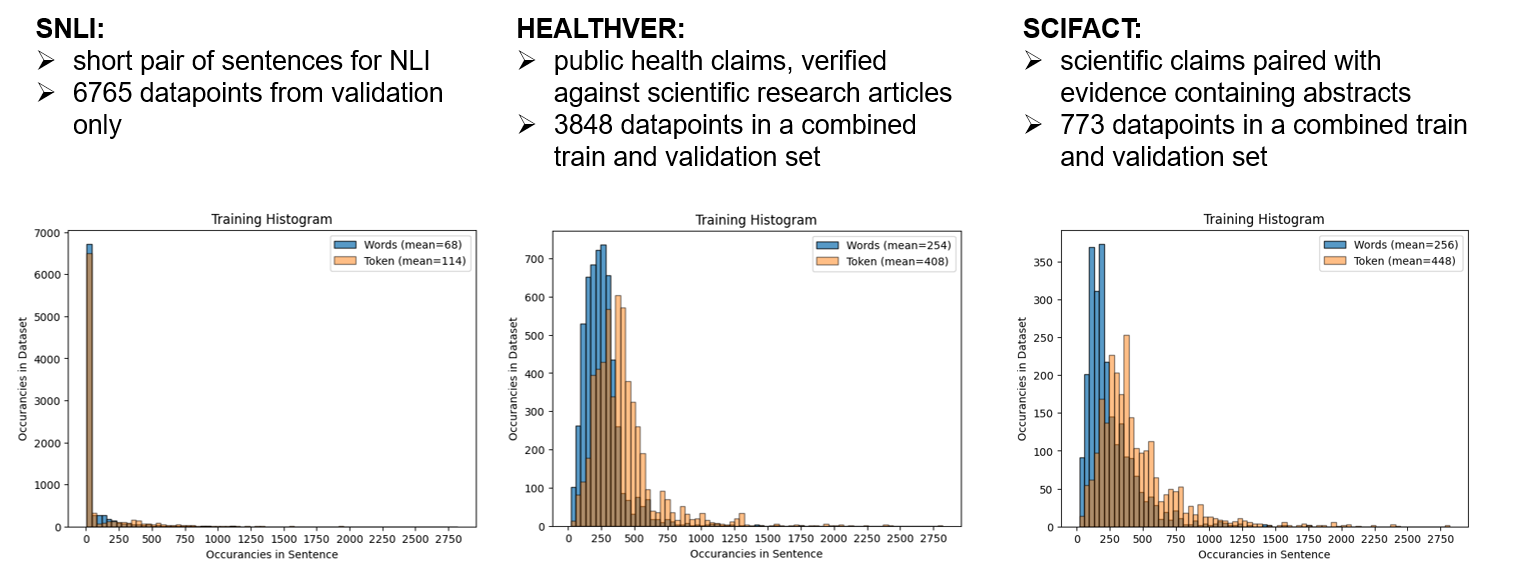
\includegraphics[width=1.3\textwidth]{./content/Histogram_Dataset.png}
    \caption{Histogram of how different Datasets combined with SemEval changes the
             Occurrences in the Bins. HEALTHVER and SCIFACT shows a slight
             shift on the x-Axis towards right, indicating that the length
             of the sentences is higher. On the other side SNLI, is dominating, 
             because the sentence structure is rather small. }
    \label{tab:histo}
\end{figure}






















